\chapter{Marco Teórico}

    \section{Fundamentos de la descarga electrostática}

        El descubrimiento de la electroestática se le atribuye a el científico griego Thales de Miletus, 
        el reporte más antiguo registrado relacionado a electricidad fue elaborado por Miletus. Thales 
        descubrió que tras frotar un trozo de ambár con pelo animal o lana
         el polvo y las hojas se veian atraidas hacia el ambár \cite{ESDA1}.
        Un dato interesante la palabra $"electro"$ viene del griego $"elektros"$ que significa ambár.

        \begin{figure}[H]
            \centering
            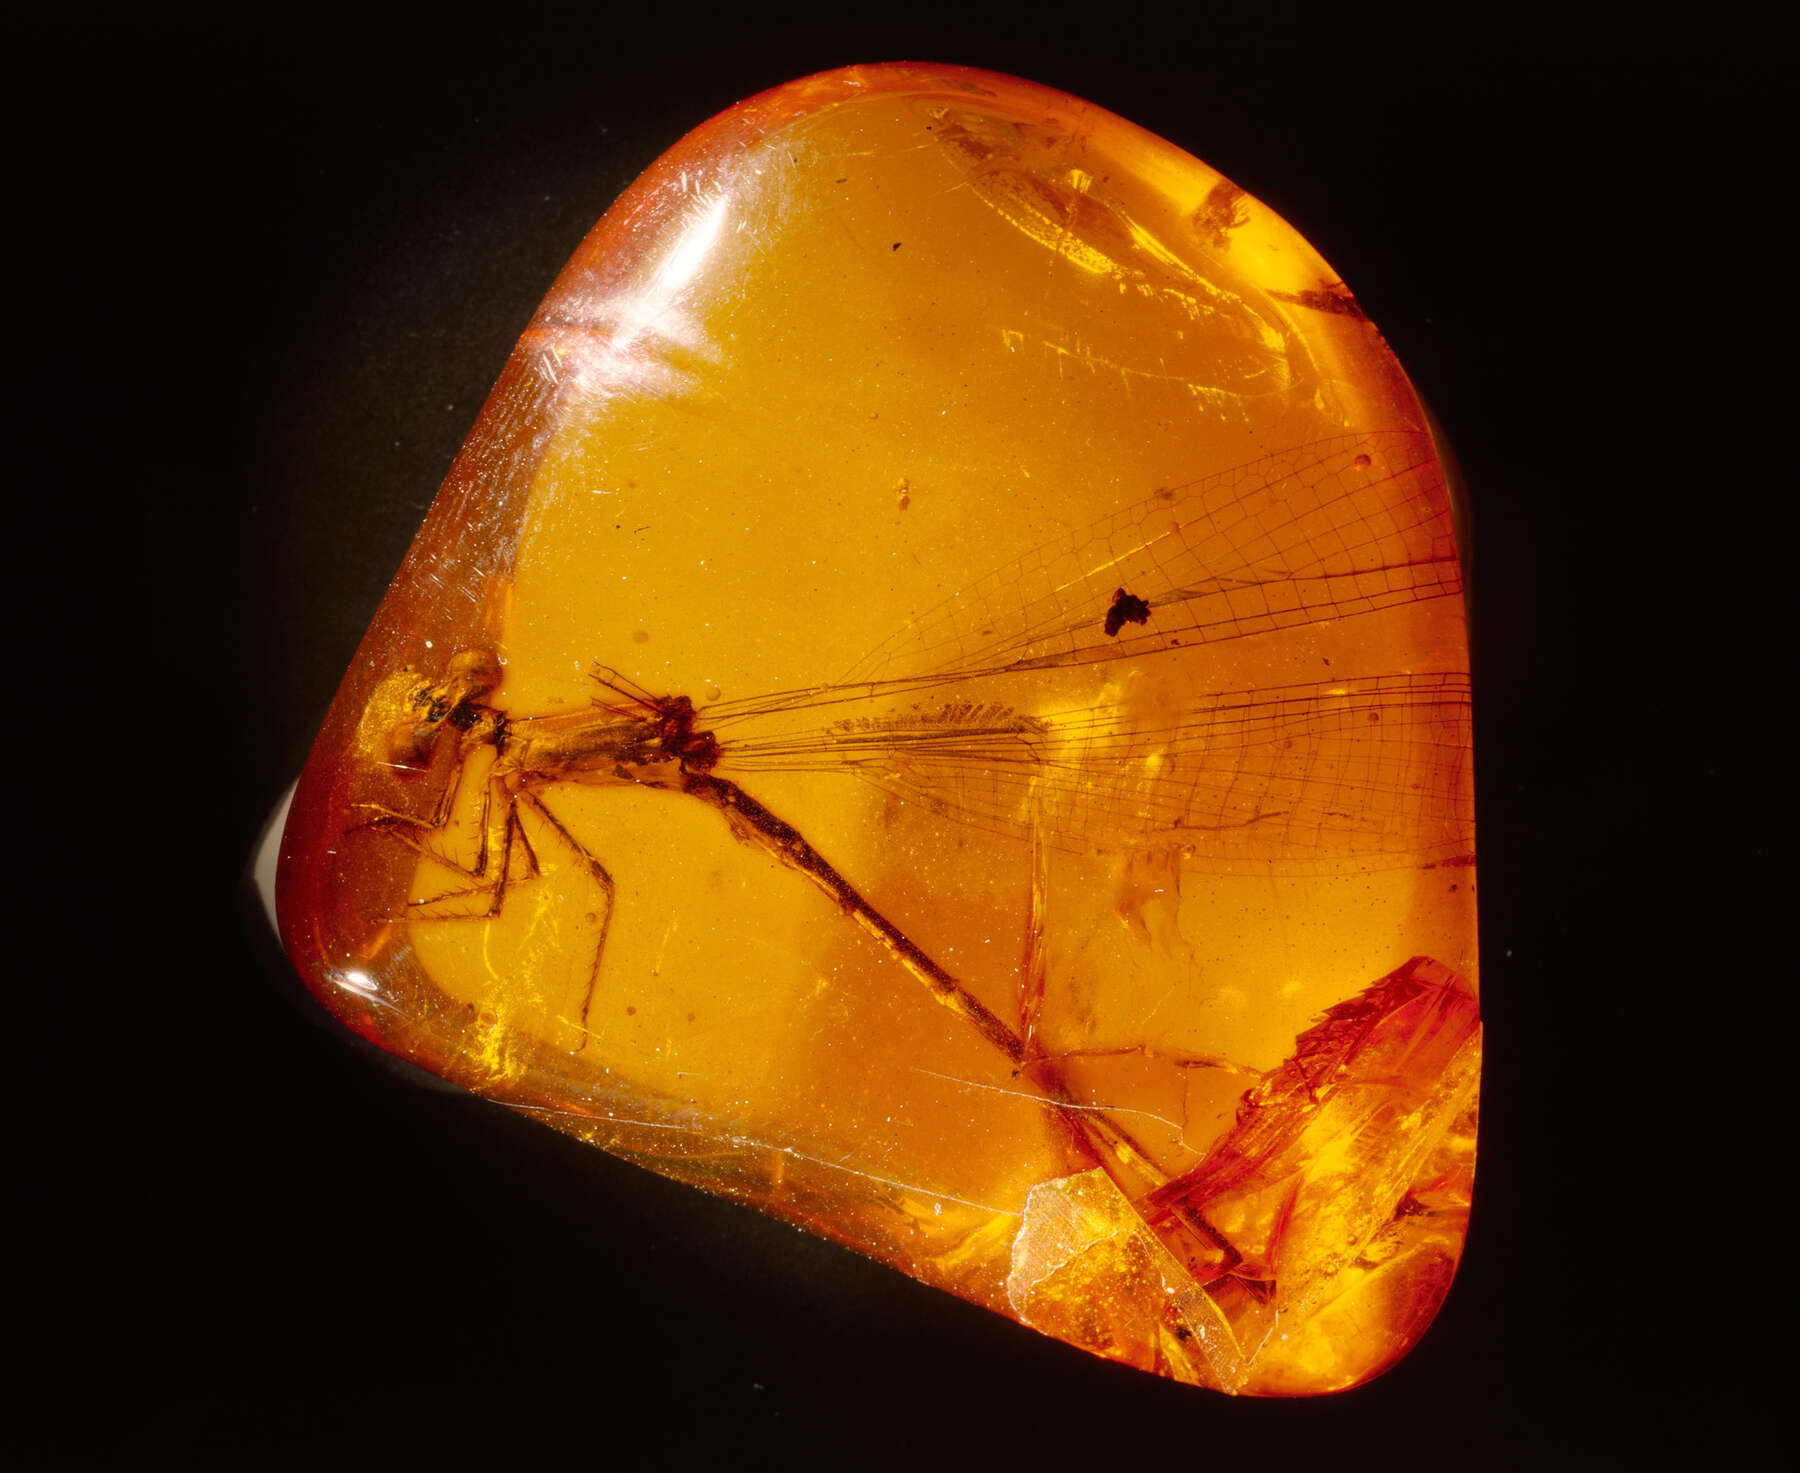
\includegraphics[width=0.4\textwidth]{pics/TF1_1.jpg}
            \caption{Fotografia de un ambár \cite{Getty_Electrostatics}}
            \label{fig:ambar}
        \end{figure}

        En ambientes muy secos es muy común que las personas experimenten $shocks$ descargas electroestáticas 
        cuando tocan algún metal de una puerta por ejemplo después de caminar por un piso alfombrado. Aunque la
        electroestática pareciera ser inofensiva, ha generado serios problemas en la industria, la electroestática 
        es capaz de dañar dispositivos electrónicos o degradar su vida útil de estos. Desde el siglo XV 
        se han iniciado a tomar medidas preventivas contra la electroestática, un ejemplo es en los fuertes
        militares Europeos y del Caribe, para evitar la ignición de los depósitos de polvora tomaban medidas
        preventivas de electroestática \cite{ESDA1}.

        \vspace{2mm}

        En la era de la electrónica, la electroestática se vuelve un problema, conforme pasan los años las compañias
        de alta tecnología crean circuitos integrados cada vez más rápidos y pequeños, lo que los hace más sensibles a 
        descargas electroestáticas, de ahi que las acciones para controlar la electroestática en ambientes donde se manipulen
        dispositivos electrónicos se ha vuelto prioritario, la electroestática afecta significativamente lo que
        las compañias productoras de circuitos integrados denominan $"yield"$, que en español se podría traducir como
        como $"rendimiento"$ \cite{ESDA1}. Ignorar la electroestática puede generar que los productos electrónicos
        que manufacture una compañia puedan ir defectuosos o del todo dañados, aunque hayan sido probados, debido a una
        descarga electroestática en el proceso de ensamblaje por ejemplo.

        \subsection{Concepto de ESD}

            La electroestática se define como cargas eléctricas en reposo, una forma sencilla de explicarlo es 
            como un desbalance de cargas eléctricas en una superficie o material, este desbalance produce un 
            campo eléctrico que puede ser medido y puede afectar otros objetos, por lo que las cargas electroestáticas
            podrían entrar dentro de la categoria de la energía potencial. Algo muy interesante de la descarga 
            electroestática es que es muy rápida, el tiempo de descarga se encuentra en el orden de pico segundos
            o nano segundos, a su vez una peculiaridad es que el campo eléctrico generado por la electroestática es muy
            alto \cite{ESDA1}, esto es lo que hace posible experimentos como el de la siguiente figura.

            \begin{figure}[H]
                \centering
                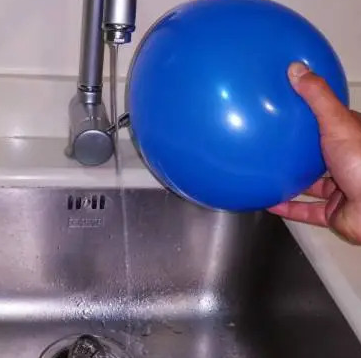
\includegraphics[width=0.4\textwidth]{pics/TF1_2.png}
                \caption{Experimento de electroestática\cite{Globos_Electrostatica}}
                \label{fig:ambar}
            \end{figure}

            Usualmente la descarga electroestática ocurre por me dio de una chispa o destello generado por la diferencia 
            entre potenciales electroestáticos entre dos objetos o cuerpos, conforme estos se van acercando esta 
            descarga aumenta. 

            \begin{figure}[H]
                \centering
                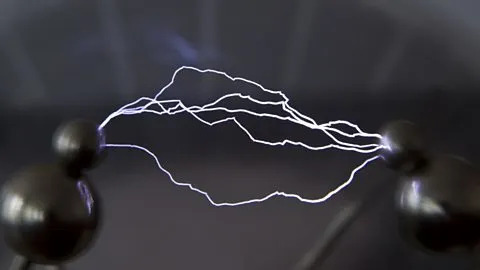
\includegraphics[width=0.5\textwidth]{pics/TF1_3.jpg}
                \caption{Chispa electroestática usando un generador de Van Graaff \cite{BBC_Static}}
                \label{fig:ambar}
            \end{figure}

            La generación de cargas electroestáticas empieza por el contacto y separación de dos materiales, lo que 
            conocemos como frotar, estos materiales pueden ser similares o asimilares, cuando son asimilares la 
            carga electroestática generada es mucho mayor. Ejemplos puede ser una persona caminando por un piso 
            alfombrado o un dispositivo electrónico deslizandose dentro o fuera de una bolsa, revista, paño, etc.

            Este tipo de generación electroestática es conocida como carga triboeléctrica, cuando los átomos de 
            dos materiales electricamente neutros tienen contacto y luego se separan estos se cargan, uno eléctricamente
            positivo y el otro electricamente negativo \cite{ESDA1}. 

            \begin{figure}[H]
                \centering
                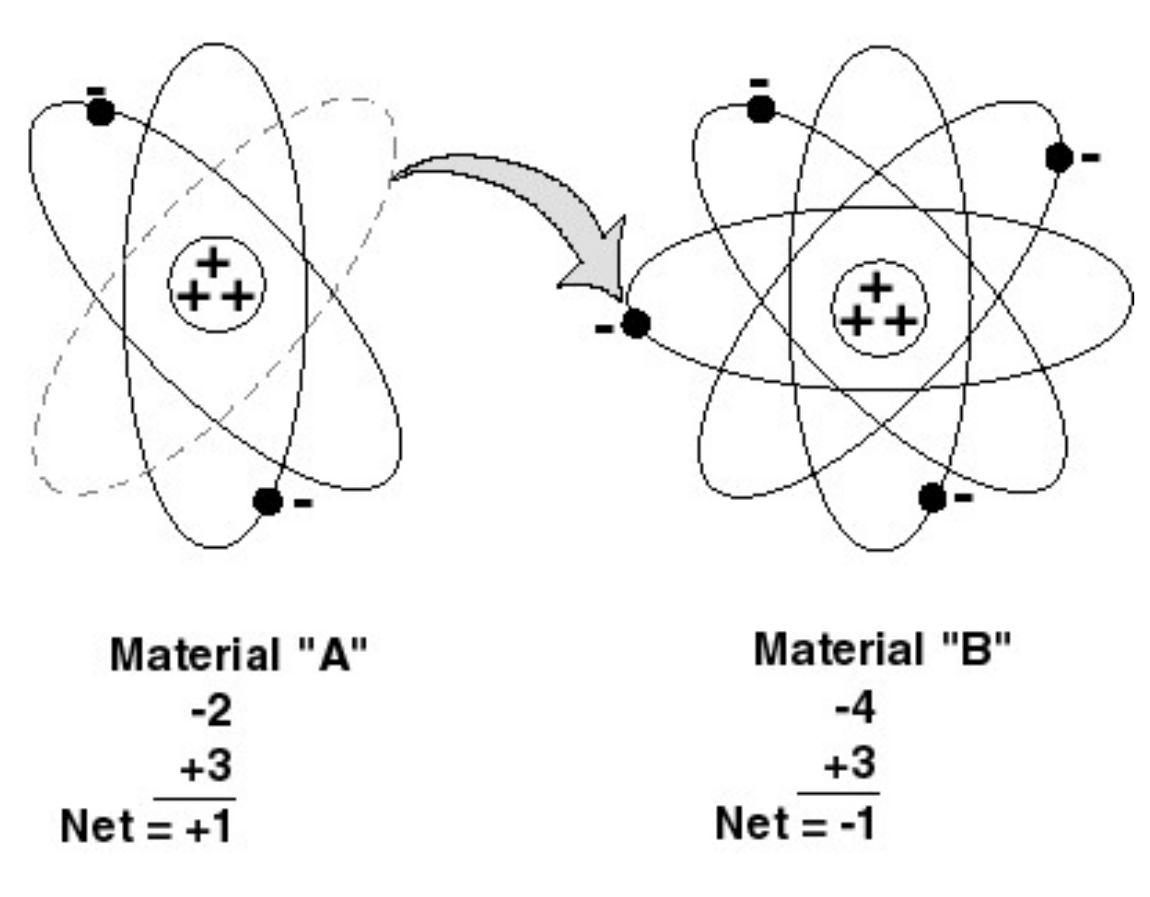
\includegraphics[width=0.55\textwidth]{pics/TF1_4.png}
                \caption{Ilustración de generación de una carga triboeléctrica \cite{ESDA1}}
                \label{fig:ambar}
            \end{figure}

            La electroestática se mide en Coulombs, comunmente se usa la ecuación de la capacitancia, donde $q$ 
            representa la cantidad de Coulombs, C la capacitancia del material, objeto o cuerpo y V el potencial 
            eléctrico:

            \begin{equation}
                q = CV
            \end{equation}

            Donde 1 Coulomb son 6.2415$\cdot 10^{18}$ cargas eléctricas, ya sean electrones o protones \cite{Illinois_Static}
            , sin embargo usualmente se habla de potencial electroestático, expresado en voltios o el campo electroestático
            expresado en voltios por metro.
            
        \subsection{Modelo de ESD HBM}
        
            Las descargas electroestáticas puede ocurrir por diferentes fuentes, debido a esto los estándares
            definen varios modelos eléctricos para representar cada caso y definir umbrales eléctricos que
            aseguren la integridad de los dispositivos electrónicos ante una descarga electroestática. Modelos como
            el HBM (Huma Body Model), CDM (Charged Device Model) y MM (Machine Model) son de los más conocidos, para 
            este proyecto nos centraremos en el HBM.

            \vspace{2mm}

            Uno de las mayores causas de daños debido a ESD es por personas, descargas electroestáticas de un
            ser humano a un material u objeto sensible a ESD. En ocaciones la carga adquirida en el cuerpo de 
            una persona puede llegar a potenciales eléctricos tan altos que puede generar una ruptura dieléctrica
            del aire, haciendo que la descarga se realize aún si haber tenido contacto pero si acercado lo suficiente
            al dispositivo afectado \cite{esda_part5}. Este modelo se conoce comunmente como HBM, que significa
            Human Body Model, es el modelo más antiguo y el modelo más utilizado para clasificar dispositivos 
            sensibles a ESD. Este modelo representa la descarga electroestática de la punta del dedo al dispositivo.

            \begin{figure}[H]
                \centering
                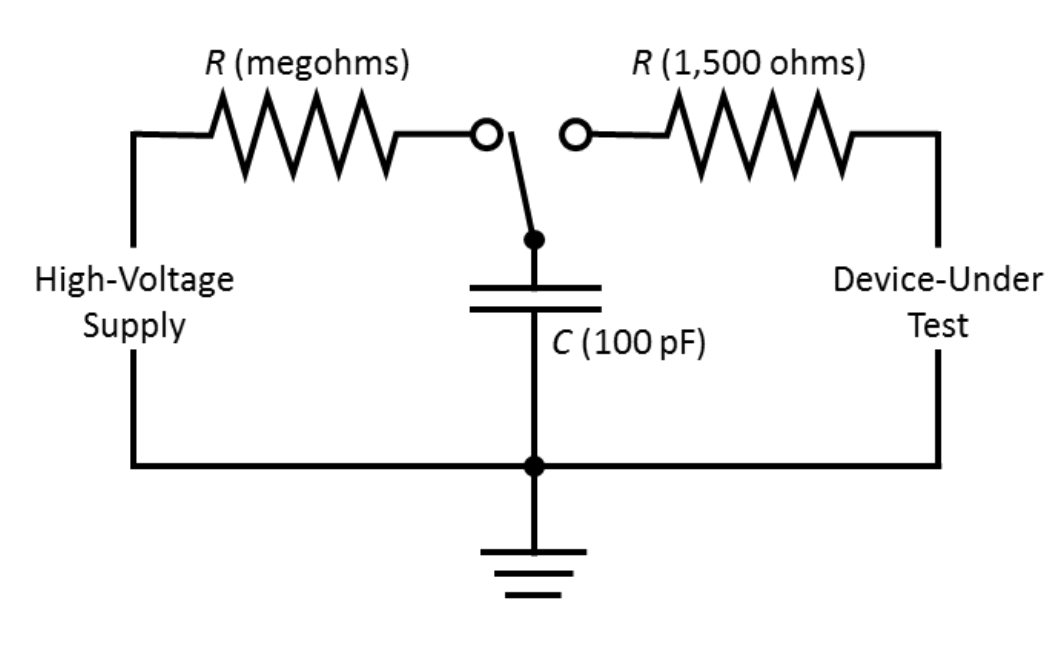
\includegraphics[width=0.55\textwidth]{pics/TF1_5.png}
                \caption{Modelo HBM simplificado \cite{esda_part5}}
                \label{fig:ambar}
            \end{figure}

            En este caso la fuente de alto voltaje representa la transferencia de cargas electroestáticas de un material
            al cuerpo, estas cargas se transfieren a nuestro cuerpo, entonces se representa con una resistencia del orden 
            de megaohms, nuestro cuerpo como tal se puede representar como una impedancia, entonces esta energia se almacena
            debido a el comportamiento capacitivo, que ronda por el orden de picofaradios, posteriormente la ruta de 
            descarga al dispositivo no suele ser directa, existe una resistencia del orden de kiloohms.

            \vspace{2mm}

            La onda de una descarga HBM se caracteriza por tener un tiempo de levantamiento entre 2-10 ns, una corriente 
            pico de 0.67 A/kV y una caida doblemente exponencial y una duración de 200 ns, la falla comúnmente se genera por
            la energia del pulso HBM \cite{esda_part5}.

            \begin{figure}[H]
                \centering
                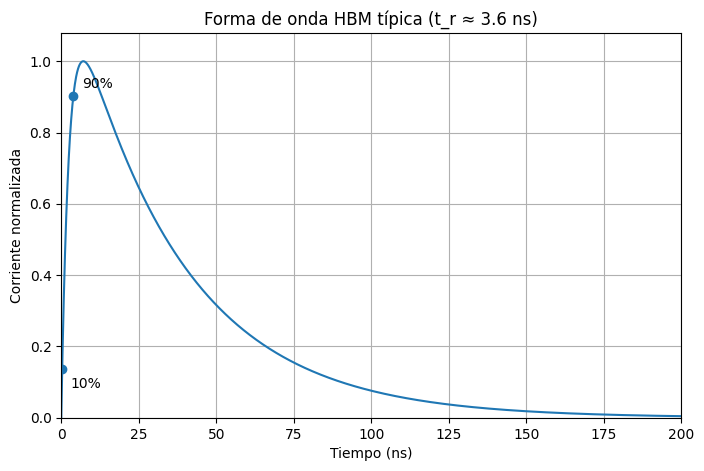
\includegraphics[width=0.65\textwidth]{pics/TF1_6.png}
                \caption{Ejemplo de un pulso HBM. Fuente: elaboración propia}
                \label{fig:ambar}
            \end{figure}

            Los dispositivos electrónicos sensibles a ESD debido al HBM se pueden clasificar según su sensibilidad, 
            distintos estándares como los ANSI/ESDA y JEDEC generan las siguientes clasificaciones:

            \begin{table}[h]
            \centering
            \caption{Clasificación de componentes ESD según el modelo HBM (ANSI/ESDA/JEDEC JS-001)}
            \begin{tabular}{|c|c|}
            \hline
            \textbf{Clasificación} & \textbf{Rango de voltaje (V)} \\
            \hline
            0Z & $< 50$ \\
            0A & $50$ a $< 125$ \\
            0B & $125$ a $< 250$ \\
            1A & $250$ a $< 500$ \\
            1B & $500$ a $< 1000$ \\
            1C & $1000$ a $< 2000$ \\
            2  & $2000$ a $< 4000$ \\
            3A & $4000$ a $< 8000$ \\
            3B & $\geq 8000$ \\
            \hline
            \end{tabular}
            \label{tab:hbm}
            \end{table}
                
            Finalmente si nos preguntaramos ¿cómo se vería un daño físico en un circuito integrado debido a una 
            descarga electroestática?, la productora de circuitos integrados Texas Instruments en uno de 
            sus reportes comparten las siguientes fotografias.

            \begin{figure}[H]
            \centering

            \begin{subfigure}[t]{0.45\textwidth}
                \centering
                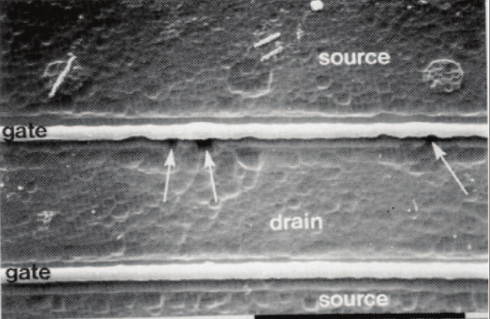
\includegraphics[width=\textwidth]{pics/TF1_7.png}
                \caption{Daño en la unión del drain y source de un transistor NMOS después de un estres HBM \cite{TI2014}}
                \label{fig:fig1}
            \end{subfigure}
            \hfill
            \begin{subfigure}[t]{0.45\textwidth}
                \centering
                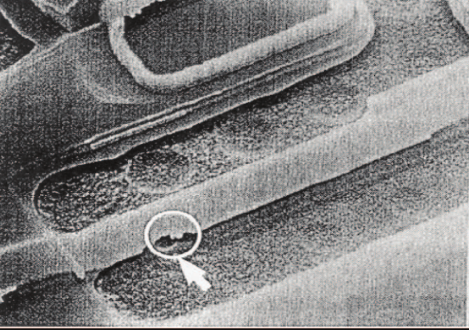
\includegraphics[width=\textwidth]{pics/TF1_8.png}
                \caption{Daño en el óxido del gate de un buffer después de un estres CDM \cite{TI2014}}
                \label{fig:fig2}
            \end{subfigure}

            \caption{Daños realizados en circuitos integrados debido a ESD}
            \label{fig:comparacion}
            \end{figure}

        \subsection{Influencia del ambiente}

            Una de las principales causas de generación de cargas electroestática en un cuerpo, material o objeto es 
            el ambiente en que esten, conforme disminuye la humedad relativa el cuerpo se aisla más de rutas para 
            descargar la energia electroestática, generando que más cargas se acumulen y por tanto se puedan llegar 
            a potenciales muy altos \cite{versalogic_esd}.

            \begin{table}[H]
                \centering
                \caption{Potenciales típicos generados en una persona según la HR y el medio}
                \begin{tabularx}{\linewidth}{Xcc}
                \toprule
                \textbf{Medio de generación} & \textbf{10--25\% HR} & \textbf{65--90\% HR} \\
                \midrule
                Caminar sobre alfombra & 35,000 V & 15,000 V \\
                Caminar sobre baldosa de vinilo & 12,000 V & 250 V \\
                Trabajar en banco & 6,000 V & 100 V \\
                Bolsa plástica levantada del banco & 20,000 V & 1,200 V \\
                Sentado en silla con espuma de uretano & 18,000 V & 1,500 V \\
                \bottomrule
                \end{tabularx}
                \label{tab:esd_humidity}

                {\small Fuente: Basado en \cite{versalogic_esd}}
            \end{table}

            Si buscaramos una explicación científica de por qué cuando la HR disminuye la cantidad de cargas electroestáticas
            en un cuerpo aumentan la respuesta es que la humedad relativa se traduce en moléculas de agua presente en el aire 
            del ambiente, estas moléculas pueden conducir las cargas electroestáticas hacia la tierra y drenarlas, es decir 
            generan un camino a tierra, por tanto se traduce en que la resistencia a tierra equivalente de la persona 
            disminuye. Cuando la humedad relativa es baja nuestro cuerpo se aisla del plano de tierra y por tanto puede 
            adquirir mayores cantidades de cargas eléctricas, esta es la razón por la que los dispositivos de control de ESD 
            se encargan de medir la resistencia del usuario a tierra, ya que si este valor se encuentra dentro de un rango 
            previamente estudiado y definido por las instituciones que han diseñado los estándares permite que la cantidad 
            de carga electroestática que genere nuestro cuerpo sea despreciable para cualquier dispositivo electrónico \cite{versalogic_esd}


    \section{Medición de resistencia cuerpo a tierra}
            Si tuvieramos que destacar uno de los conceptos más importantes de este proyecto, la medición resistiva del 
            cuerpo a tierra, o comúnmente conocida en inglés como Body to Ground Resistence entraria en esta lista. En un 
            laboratorio este plano a tierra seria la superficie del piso, entonces lo que se busca es que el usuario tenga 
            una resistencia eléctrica de su cuerpo a la superficie del piso que este dentro de un rango específico en el orden 
            de los M$\Omega$ \cite{STM97_ANSI}.

            \begin{figure}[H]
                \centering
                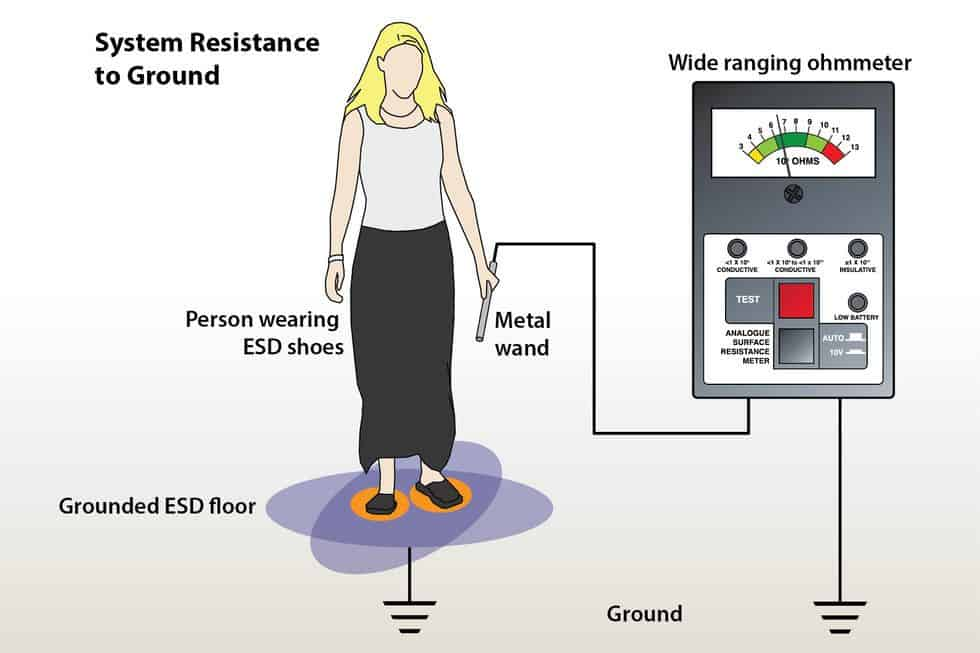
\includegraphics[width=0.65\textwidth]{pics/TF2_1.jpg}
                \caption{Ilustración de medición de resistencia de cuerpo a tierra \cite{STM97_ANSI}}
                \label{fig:resistencia_a_tierra}
            \end{figure}

            Esta medición se debe hacer con estimulos eléctricos en DC, las normas lo establecen de esta manera, un punto 
            importante es que nuestro cuerpo modelado como impedancia se podría representar de la siguiente manera:

            \begin{equation}
                Z_{Cuerpo} = R\text{(f)} + jX\text{(f)}
            \end{equation}

            Por lo que el componente resistivo depende de la frecuencia de la señal de estimulo que se aplique, lo mismo 
            ocurre con la reactancia. La reactancia de nuestro cuerpo es capacitiva, esto es un punto importante ya que 
            es la capacitancia de nuestro cuerpo lo que permite almacenar la energia electroestática, como se puede observar 
            en el modelo HBM \cite{dtic_skin}. Para fines médicos es común el estudio de la impedancia del cuerpo desde diferentes 
            sectores, sin embargo para fines de este proyecto no es relevante, por eso se elije $f=0$ Hz como punto de 
            medición a utilizar.
            
    \section{Medición de alta impedancia}

        Un dispositivo de control ESD debe ser preciso en su medición, esto no es una tarea fácil cuando hablamos de valores 
        entre a 750 k$\Omega$ a 35 M$\Omega$, dispositivos como el Desco 19240 realizan estas mediciones con una precisión de 
        $\pm 10$ para 750 k$\Omega$ y $\pm 15$ para 10 M$\Omega$. Debido a que los valores de impedancia son tan altos esto 
        se traduce en corrientes de $\mu$A , por lo que corrientes de fuga en la PCB o usar componentes con impedancias 
        que no sean lo suficientemente altas pueden generar errores. Debido a esto se usará el libro
        ofrecido por Tektronix sobre técnicas para mediciones de bajo nivel \cite{keithley_lowlevel}
        \subsection{Corrientes de fuga}

            Cuando se va a medir una alta impedancia entra en juego las corrientes de fuga, estas corrientes suelen ser 
            del orden de $\mu$A o nA, sin embargo es suficiente para generar errores de hasta o mayores a un 10\% en la medición,
            por ejemplo:

            \begin{align}
                R = \frac{V}{I}, \hspace{2mm} I = I_{DUT} + I_{fuga}
            \end{align}

            Si la corriente medida es de 1 $\mu$A y la corriente de fuga es de 100 nA eso implica un error de un 10\% en la 
            medición, una fuga de 100 nA por ejemplo es un valor bastante probable de tener en la práctica, de ahi la importancia 
            de considerar estas corrientes en el diseño del circuito y PCB \cite{keithley_lowlevel}. Para poder contrarestar esto 
            es necesario utilizar buenos materiales aislantes en el diseño PCB, reducir los niveles de humedad en el ambiente y 
            usar técnicas de guardado. Cuando hay altos niveles de humedad los materiales aislantes presentes en el circuito 
            pueden absorber el agua del agua y generar contaminantes ionicos que causan corrientes espurias. Materiales a utilizar 
            son teflon y polietileno, sin embargo se debe evitar los fenólicos y el nylos \cite{keithley_lowlevel}.

            \begin{figure}[H]
                \centering
                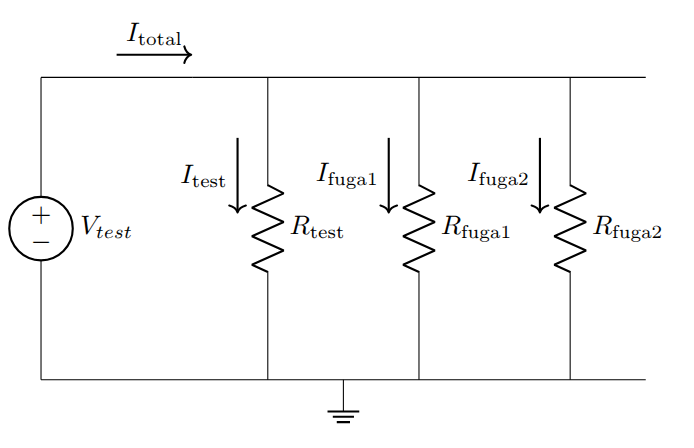
\includegraphics[width=0.65\textwidth]{pics/TF3_1.png}
                \caption{Ilustración de corrientes de fuga. Fuente: elaboración propia}
                \label{fig:resistencia_a_tierra}
            \end{figure}

            En la siguiente figura 
            se muestran rangos típicos de corriente generadas por distintas fuentes de fuga, como por ejemplo el 
            ruido presente en la electrónica o bien que pueden generar ciertos materiales, 
            esto puede darnos una idea de que materiales evitar.

            \begin{figure}[H]
                    \centering
                    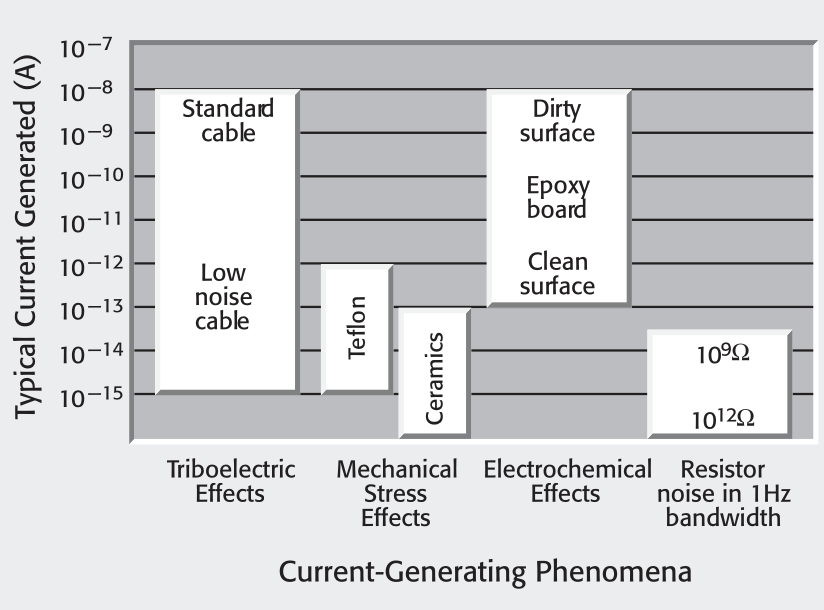
\includegraphics[width=0.65\textwidth]{pics/TF4_1.png}
                    \caption{Valores típicos de corrientes generadas por ruido \cite{keithley_lowlevel}}
                    \label{fig:resistencia_a_tierra}
            \end{figure}

            En \cite{keithley_lowlevel} se muestra una técnica para contrarestar estas corrientes de fuga, si fuese 
            posible aproximar su valor de pérdida o bien caracterizar el circuito de medición se podría contrarestar este
            efecto, ya sea a manera de hardware o software.

            \begin{figure}[H]
                    \centering
                    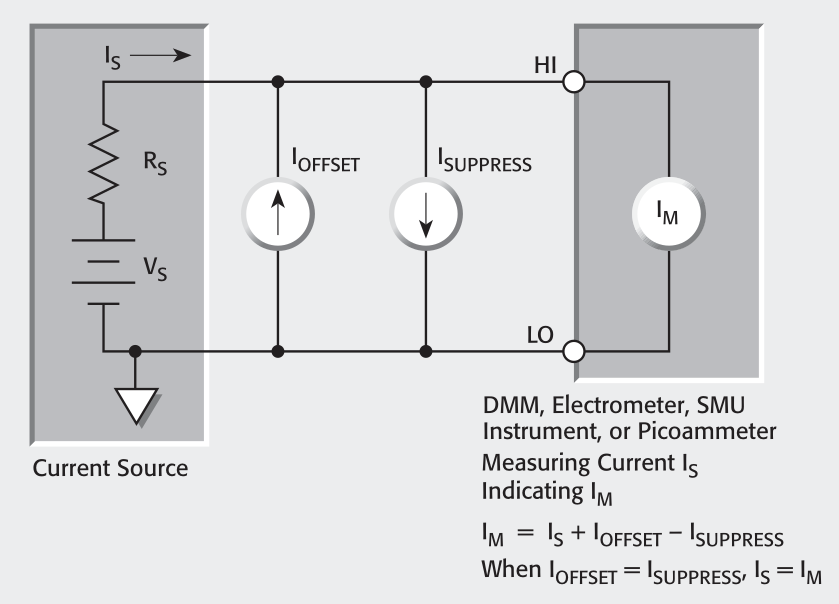
\includegraphics[width=0.65\textwidth]{pics/TF4_2.png}
                    \caption{Uso de fuente externa para suprimir corrientes de fuga \cite{keithley_lowlevel}}
                    \label{fig:resistencia_a_tierra}
            \end{figure}


        \subsection{Técnicas de guardado (guarding)}

            Una forma de evitar las corrientes de fuga es forzando los potenciales eléctricos de los sectores hacia donde fluyen
            estas corrientes al mismo de la señal de estimulo aplicada, un ejemplo es se observa con el siguiente cable 
            triaxial, el cual la primer capa se conecta al mismo potencial del pin del cable, generando una diferencia de 0 V
            entre la trayectoria, y por tanto eliminando o disminuyendo significativamente la corriente de fuga.

            \begin{figure}[H]
                \centering
                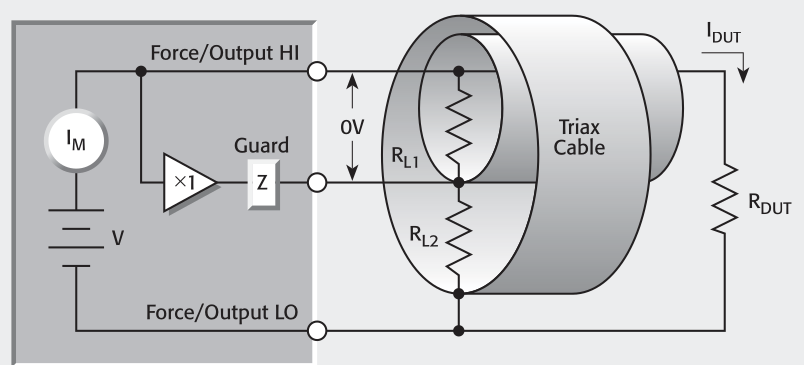
\includegraphics[width=0.65\textwidth]{pics/TF3_2.png}
                \caption{Aplicación de técnica de guardado en cable triaxial \cite{keithley_lowlevel}}
                \label{fig:resistencia_a_tierra}
            \end{figure}

            \begin{figure}[H]
                \centering
                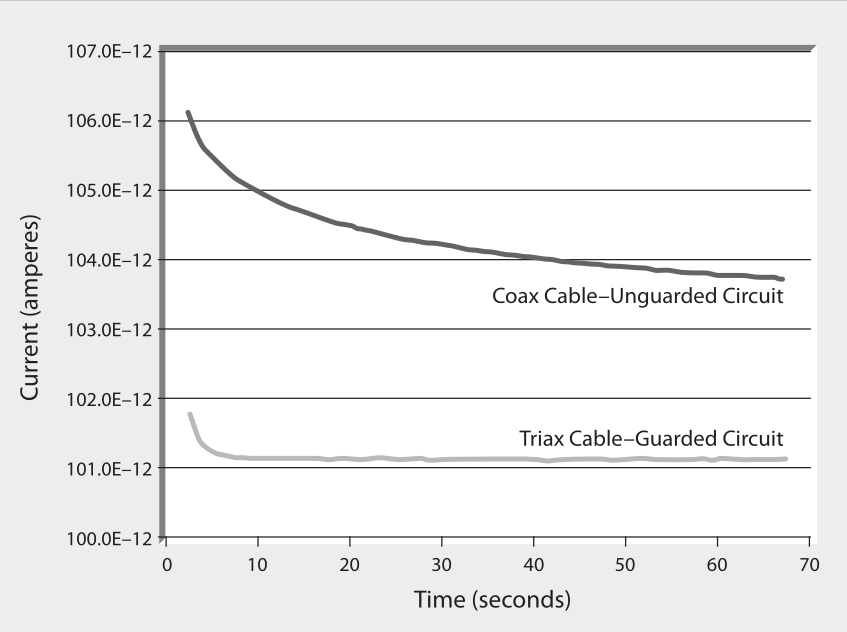
\includegraphics[width=0.65\textwidth]{pics/TF3_3.png}
                \caption{Resultados obtenidos tras usar la técnica de guardado tras medir una resistencia de 100 M$\Omega$ \cite{keithley_lowlevel}}
                \label{fig:resistencia_a_tierra}
            \end{figure}

        \subsection{Circuitos para medición de altas impedancias}

            Los circuitos para medir altas impedancias no suelen ser complejos, pero sí precisos, los componentes a 
            utilizar deben de ser capaces de medir corrientes en el orden de $\mu$A o hasta nA. Uno de los componentes 
            más conocidos en esta área de la electrónica es el electrometer o picoammeter, es principalmente conocido 
            por su nombre en inglés \cite{keithley_lowlevel}. Estos circuitos integrados son similares a un 
            amplificador operacional, sensibles usualmente a pA, de ahi su nombre, un circuito de ejemplo es el siguiente.

            \begin{figure}[H]
                \centering
                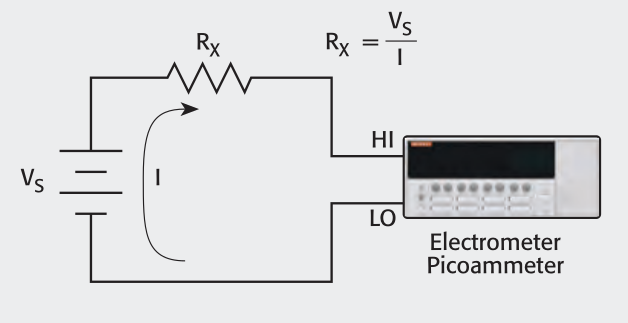
\includegraphics[width=0.65\textwidth]{pics/TF4_3.png}
                \caption{Circuito de medición de resistencia con un electrometer \cite{keithley_lowlevel}}
                \label{fig:resistencia_a_tierra}
            \end{figure}

            Este circuito medirá el valor de $I$, esto lo convertirá en tensión eléctrica que podrá ser medida con un ADC de 
            alta precisión para luego enviarse a un microcontrolador. 

            Es posible también construir un electrometer, utilizando técnicas de guardado en \cite{keithley_lowlevel}
            muestran la siguiente propuesta.

            \begin{figure}[H]
                \centering
                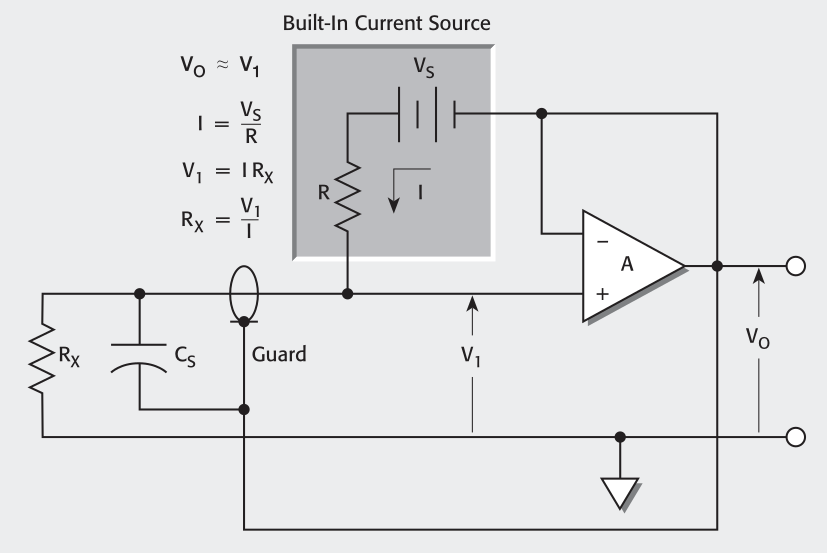
\includegraphics[width=0.65\textwidth]{pics/TF4_4.png}
                \caption{Circuito de medición de resistencia con un electrometer sin IC \cite{keithley_lowlevel}}
                \label{fig:resistencia_a_tierra}
            \end{figure}

            Otra opción es medir la tensión generada en la resistencia tras aplicar una corriente conocida y luego utilizando 
            un voltimetro o bien un ADC de alta precisión.

            \begin{figure}[H]
                \centering
                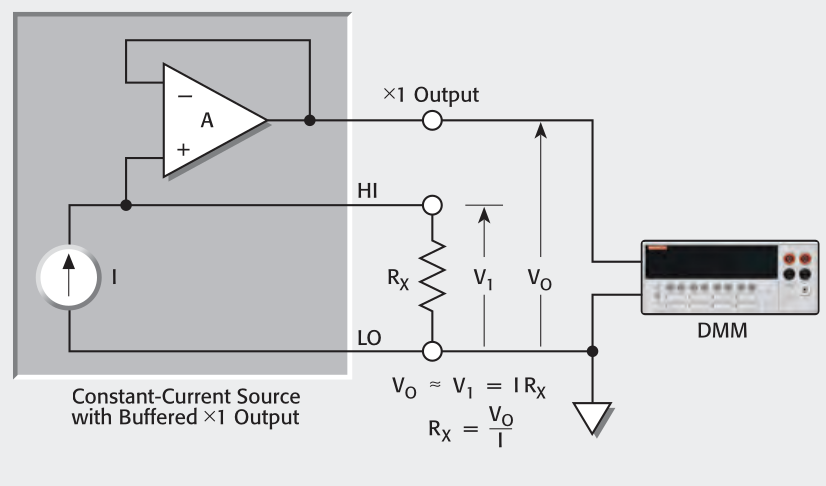
\includegraphics[width=0.65\textwidth]{pics/TF4_5.png}
                \caption{Medición de resistencia utilizando fuente de corriente \cite{keithley_lowlevel}}
                \label{fig:resistencia_a_tierra}
            \end{figure}

            Usando la Ley de Ohm y un dividor de tensión también es posible obtener la medición.

            \begin{figure}[H]
                \centering
                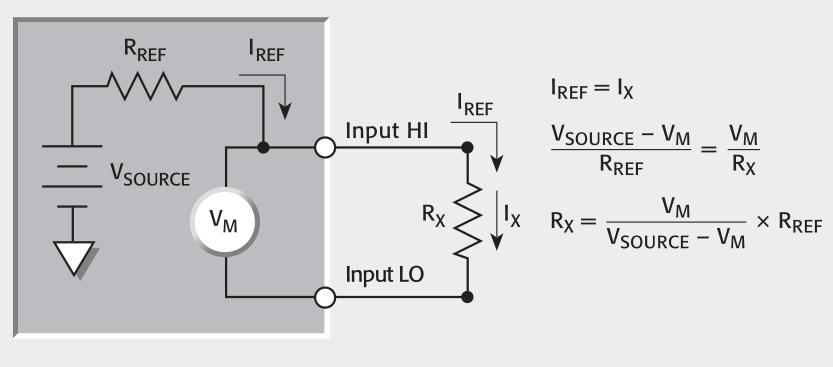
\includegraphics[width=0.65\textwidth]{pics/TF4_6.png}
                \caption{Medición de resistencia utilizando fuente de tensión\cite{keithley_lowlevel}}
                \label{fig:resistencia_a_tierra}
            \end{figure}

            Finalmente si se deseara mucha más precisión se podría optar por el diseño de un electrómetro digital.

            \begin{figure}[H]
                \centering
                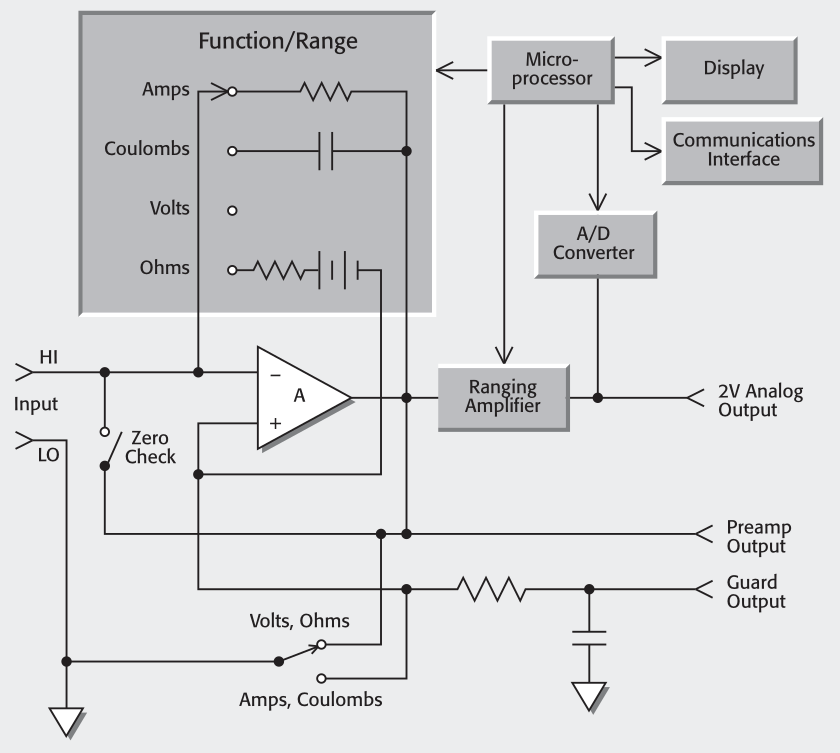
\includegraphics[width=0.65\textwidth]{pics/TF4_7.png}
                \caption{Eletrometro digital típico \cite{keithley_lowlevel}}
                \label{fig:resistencia_a_tierra}
            \end{figure}

\chapter{Estado del Arte}

    \section{Sistemas ESD en la literatura}

        En la literatura se han propuesto diversos sistemas para control ESD, sin embargo estos estan
        orientados a el monitoreo continuo de puesta a tierra por medio del IoT o bien otras referencias
        se centran en la medición de presencia de carga electroestática en el cuerpo humano, en 
        circuitos integrados y tarjetas electrónicas.

        En el trabajo de \cite{Nagy2025} se propone un sistema de monitoreo continuo de puesta a tierra por medio del IoT,
        este sistema se compone te un servidor y modulos en estaciones de trabajo, los modulos estan continuamente midiendo
        la resistencia de el usuario a tierra, comparandola con un umbral, en caso de que este umbral se supere envia una alerta
        al servidor. El trabajo se centra en diseñar la tarjeta electrónica del servidor, no se extiende a el diseño de los módulos.

        \begin{figure}[H]
            \centering
            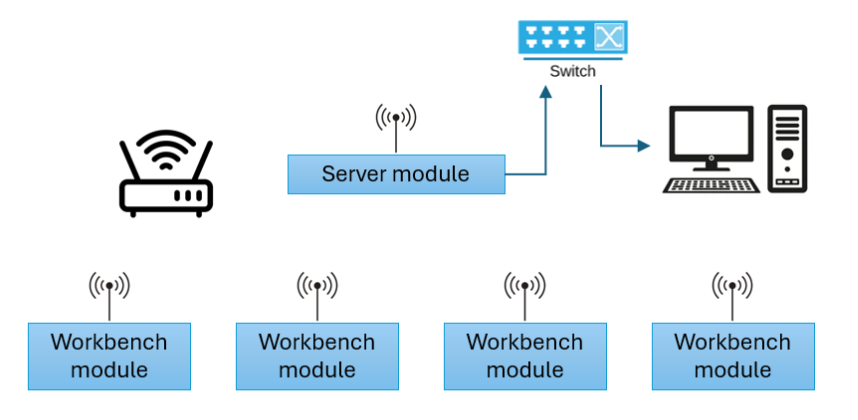
\includegraphics[width=0.8\textwidth]{pics/SA1_01.png}
            \caption{Diagrama de bloques del sistema propuesto por Nagy \cite{Nagy2025}.}
            \label{fig:nagy2025}
        \end{figure}

        \begin{figure}[H]
            \centering
            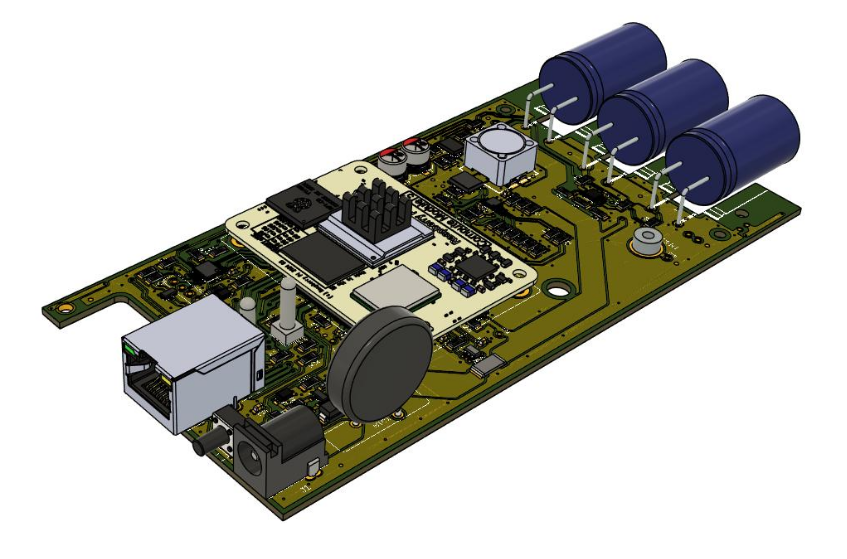
\includegraphics[width=0.8\textwidth]{pics/SA1_02.png}
            \caption{Diseño de la tarjeta electrónica para el servidor por Nagy \cite{Nagy2025}.}
            \label{fig:nagy2025_2}
        \end{figure}

        En el trabajo de Xu \cite{Xu2023} se diseña un sistema de medición de presencia de carga electróestática en tarjetas electrónicas
        o lineas de producción de manufactura de dispositivos electrónicos, esto se logra por medio de lectores de campos eléctricos instalados en
        la linea de producción, usando motores y sistemas mecánicos el sistema posiciona el lector en puntos estratégicos de la linea, las mediciones
        se digitalizan y envian a un servidor.

        \begin{figure}[H]
            \centering
            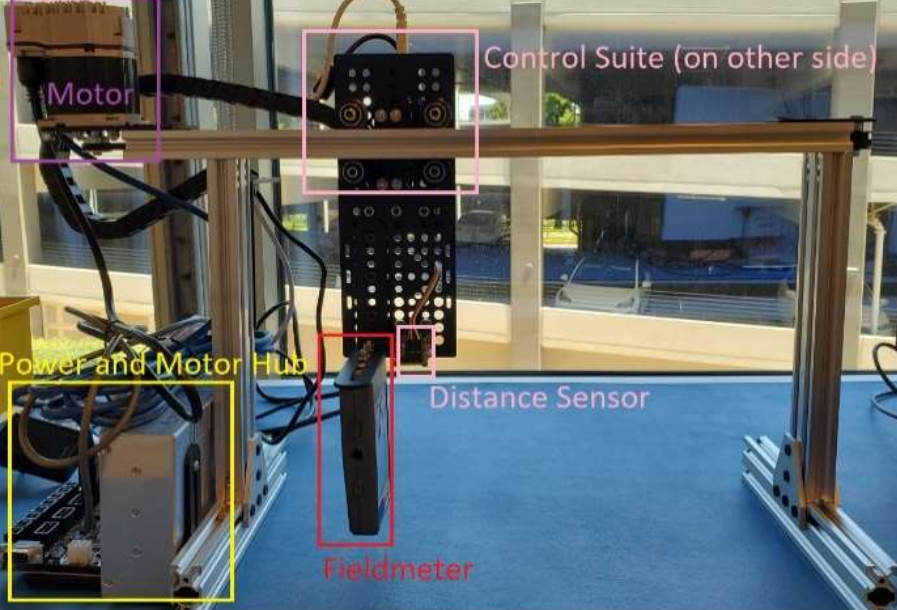
\includegraphics[width=0.8\textwidth]{pics/SA1_03.png}
            \caption{Sistema propuesto por Xu \cite{Xu2023}.}
            \label{fig:xu2023}
        \end{figure}

        Luego en el trabajo de Raúl \cite{URV2023} se automatiza un test de ESD en dispositivos electrónicos 
        automotrices, el test consiste en inyectar una descarga electroestática a un dispositivo electrónico
        y medir su respuesta, anteriormente este test se realizaba manualmente, Raúl automatiza el test
        por medio de un brazo robótico.

    \section{Implementaciones de medición de resistencia en sistemas ESD}

        El circuito electrónico principal en un sistema de control ESD es el 
        circuito encargado de medir la resistencia del usuario a tierra. Actualmente no
        existen circuitos integrados del tipo front-end diseñados específicamente para esta
        aplicación, aunque la medición de resistencia de alta impedancia es un tema común en la electrónica.
        Tampoco los fabricantes de sistemas ESD comerciales publican detalles de sus circuitos electrónicos, 
        entonces la pregunta sería, ¿cómo se mide la resistencia de alta impedancia en sistemas ESD?.
        
        \vspace{2mm}

        Lo más cercano que se puede encontrar en el mercado son IC como el
        AD5933 de Analog Devices, este IC es un convertidor analógico a digital de impedancia con
        un rango de 1 k$\Omega$ a 10 M$\Omega$, usando señales alternas de estimulo con frecuencias entre
        1 kHz y 100 kHz \cite{AD5933}. Sin embargo el AD5933 no esta diseñado específicamente para la medición 
        de resistencia de alta impedancia DC, debido a que la resistencia del cuerpo a tierra depende de la 
        frecuencia de la señal del estimulo generaria una medición inexacta, almenos que se usen frecuencias
        muy bajas, limitante que tiene este IC. 

        \begin{figure}[H]
            \centering
            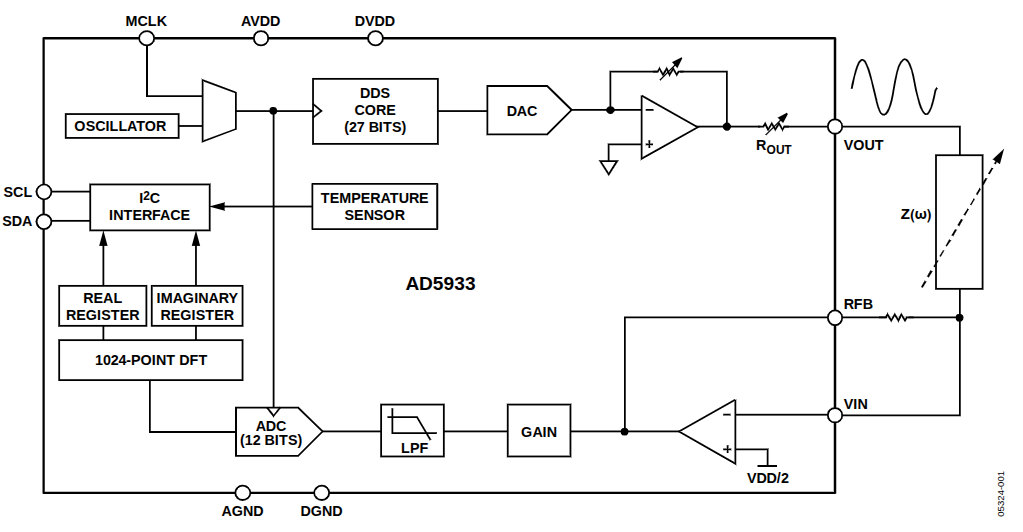
\includegraphics[width=0.6\textwidth]{pics/SA1_04.png}
            \caption{Diagrama de bloques del AD5933 \cite{AD5933}.}
            \label{fig:ad5933}
        \end{figure}

        También existen IC como el ICL7106 de Analog Devices, este IC entra dentro de la categoria de IC 
        para DMM (digital multimeter) este IC es un convertidor analógico a digital de 3.5 dígitos, 
        con un rango de medición de hasta 200 M$\Omega$ \cite{ICL7106}. Sin embargo en comparación con el AD5933, el ICL7106 
        no tiene puertos de comunicación digital, lo que dificulta su integración en un sistema de control ESD. Este IC esta
        diseñado para ser usado con un display LCD. Si se deseara usar este IC se deberá tener un decodificador de display LCD.

        \begin{figure}
            \centering
            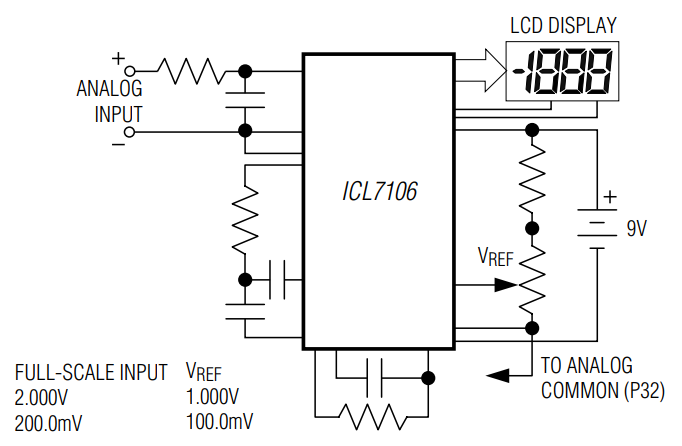
\includegraphics[width=0.6\textwidth]{pics/SA1_05.png}
            \caption{Circuito de operación típico del ICL7106 \cite{ICL7106}.}
            \label{fig:icl7106}
        \end{figure}

        Las siguientes opciones requiere de diseñar un circuito electrónico de precisión para realizar la medición, 
        usando amplificadores operacionales de muy baja corriente de fuga, técnicas de guardado (guarding) 
        y técnicas de cancelación de ruido. A su vez dispositivos como DAC (digital to analog converter) 
        y ADC (analog to digital converter) de alta resolución para generar la señal de estimulo y 
        digitalizar la medición respectivamente. Este tipo de soluciones no estan disponibles comercialmente, 
        no existen tarjetas electrónicas de desarrollo o módulos que implementen este tipo de circuitos, 
        entonces se deberá diseñar el circuito electrónico desde cero usando los dispositivos electrónicos
        comentados anteriormente.

    \section{Normativas aplicables a sistemas ESD}

        Los estándares aplicables a sistemas de control ESD son principalmente los siguientes:
        \begin{table}[H]
        \centering
        \caption{Principales normativas aplicables a sistemas de control ESD}
        \begin{tabular}{|l|p{10cm}|}
        \hline
        \textbf{Norma} & \textbf{Descripción} \\
            \hline

            ANSI/ESD S20.20 &
            Establece los requisitos para implementar un programa completo 
            de control ESD en entornos industriales. 
            Define procedimientos para la puesta a tierra del personal, 
            control de materiales y verificación de cumplimiento \cite{ANSI_S2020_Blog}. \\
            \hline

            IEC 61340-5-1 &
            Norma internacional que especifica los requisitos generales 
            para la protección contra descargas electrostáticas en áreas 
            protegidas (EPA), incluyendo métodos de medición 
            y control de resistencias \cite{IEC61340_Preview}. \\
            \hline

            ANSI/ESD STM97.1 &
            Define el método de medición de la resistencia del sistema 
            persona-calzado-suelo, utilizado para evaluar la efectividad 
            de la puesta a tierra del operador mediante calzado ESD \cite{STM97_ANSI}. \\
            \hline

            ANSI/ESD S1.1 &
            Establece el método de prueba para pulseras antiestáticas 
            (wrist straps), incluyendo los rangos aceptables de resistencia 
            para garantizar una correcta disipación de carga \cite{S1_1_ANSI}. \\
            \hline

            IEC 61000-4-2 &
            Describe el método de ensayo de inmunidad a descargas 
            electrostáticas a nivel de sistema, simulando eventos ESD 
            para evaluar la robustez de equipos electrónicos \cite{IEC61000_ITU}. \\
            \hline

            JEDEC JS-001 &
            Define el modelo de descarga del cuerpo humano (HBM) 
            para la caracterización de la susceptibilidad ESD 
            en dispositivos semiconductores a nivel de componente \cite{JEDEC_JTR001}. \\
            \hline

            IEC60479 &
            Define los estimulos eléctricos aplicables a un ser humano
            , lo que involucra limites de corriente y tensión para que 
            el dispositivo sea seguro para el usuario. \cite{IEC60479}. \\
            \hline

        \end{tabular}
        \label{tab:esd_normas}
        \end{table}

        De estos los más relevantes para el diseño de un sistema de control ESD para laboratorios de electrónica 
        son el ANSI/ESD S20.20, IEC 61340-5-1, ANSI/ESD STM97.1, IEC60479 y ANSI/ESD S1.1, 
        ya que estos estándares establecen los requisitos para la puesta a tierra del personal, 
        control de materiales y verificación de cumplimiento, así como los métodos de medición de 
        la resistencia del sistema persona-calzado-suelo y pulseras antiestáticas. Un limitante 
        importante es que estas normativas no estan disponibles gratuitamente, 
        por lo que el contenido disponible son resúmenes o extractos de las mismas. Sin embargo existen
        organizaciones como la ESD Association que publican resúmenes y articulos relacionados a las normativas.
        \vspace{2mm}

        De los estándares mencionados la información más importante se resumen en una resistencia de 
        puesta a tierra menor a 35 M$\Omega$ y mayor a 750 k$\Omega$ (en el caso de la muñequera debe
        ser menor a 10 $\Omega$) para el sistema persona-calzado-suelo 
        y pulseras antiestáticas, este rango de valores asegura una correcta disipación de carga
        electroestática y a su vez protege al usuario de corrientes peligrosas \cite{IEC61340_Preview}. A su vez
        la corriente máxima aplicable a un usuario para que este no tenga percepción de la descarga es de 1 mA \cite{IEC60479}.
        

    \section{Sistemas comerciales de control ESD}

        Actualmente existen diversos sistemas comerciales de control ESD, desde dispositivos económicos para medición del
        correcto funcionamiento de pulseras antiestáticas, hasta sistemas inteligentes creados para entradas de manofactura
        de dispositivos electrónicos. 

        Desco Industries ofrece su producto Desco 19240, este dispositivo es un tester de pulseras antiestáticas, 
        el dispositivo tiene un costo de 150 USD \cite{Desco_19240}, este dispositivo se limita a dar 3 resultados, 
        $"Pass"$, $"Fail"$ o $"Open"$, dependiendo de la resistencia medida, 
        el dispositivo no tiene capacidad de comunicación digital, 
        lo que dificulta su integración en un sistema de control ESD inteligente.

        \begin{figure}[H]
            \centering
            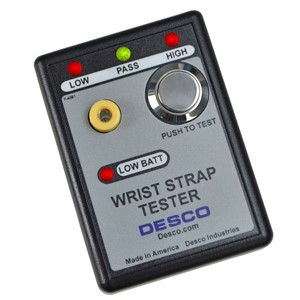
\includegraphics[width=0.4\textwidth]{pics/SAL4_01.jpg}
            \caption{Tester de pulseras antiestáticas Desco 19240 \cite{Desco_19240}.}
            \label{fig:desco19240}
        \end{figure}

        La empresa SCS, la cual es parte de Desco Industries, ofrece su producto 770758 Dual Combination Wrist 
        Strap and Footwear Tester, este dispositivo es un tester para verificar simultáneamente 
        la resistencia de pulseras antiestáticas y calzado ESD, el dispositivo tiene un costo de 1181 USD \cite{SCS_770758}, 
        este dispositivo también se limita a dar resultados de $"Pass"$ o $"Fail"$ dependiendo de la resistencia medida, 
        y tampoco tiene capacidad de comunicación digital.

        \begin{figure}[H]
            \centering
            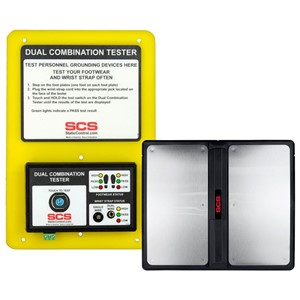
\includegraphics[width=0.4\textwidth]{pics/SAL4_02.jpg}
            \caption{Tester de pulseras antiestáticas Desco 19240 \cite{Desco_19240}.}
            \label{fig:desco19240}
        \end{figure}
        
        Luego tenemos a la empresa Transforming Technologies, la cual ofrece su producto PGT120 Combination 
        ESD Tester for Personal Grounding Equipment, este tiene un costo de 2137 USD \cite{PGT120} este dispositivo es muy similar a el SCS 770758, 
        pero con la diferencia que puede generar control de acceso abriendo una puerta o barrera. Transforming Technologies
        tiene un modelo más avanzado PGT130 el agrega lectura RFID y generación de reportes, con un costo de 
        7676 USD \cite{PGT130DT}.
            \begin{figure}[H]
            \centering

            \begin{subfigure}[t]{0.45\textwidth}
                \centering
                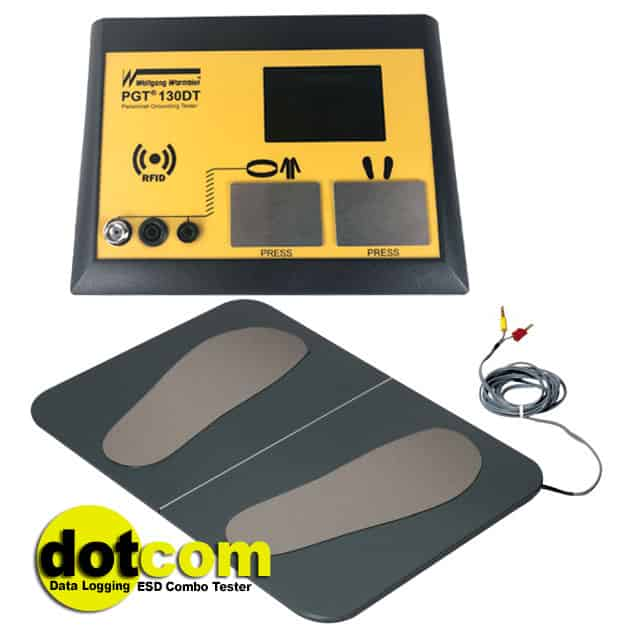
\includegraphics[width=\textwidth]{pics/SAL4_03.jpg}
                \caption{PGT130 \cite{PGT130DT}}
                \label{fig:fig1}
            \end{subfigure}
            \hfill
            \begin{subfigure}[t]{0.45\textwidth}
                \centering
                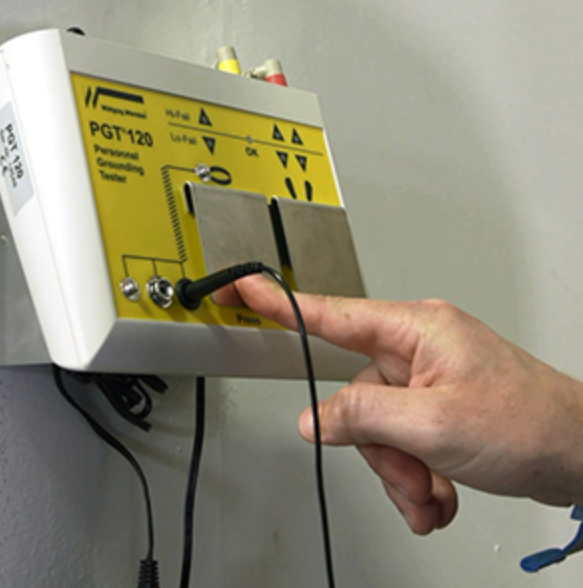
\includegraphics[width=\textwidth]{pics/SAL4_04.png}
                \caption{PGT120 \cite{PGT120}}
                \label{fig:fig2}
            \end{subfigure}

            \caption{Modelos PGT de Transforming Technologies}
            \label{fig:comparacion}
            \end{figure}


        Finalmente tenemos los sistemas inteligentes de control ESD como el ESDMAN ESD Access Control System, con un costo
        de 2500 USD en su versión básica \cite{ESDMAN_0016809} y la empresa Desco Industries ofrece su producto
        SmartLog Pro 2 con un precio inicial de 5643 USD \cite{Desco_19240}. Ambos realizan medición de pulsera y calzado,
        a su vez tienen lector RFID, un sistema de generación de reportes y control de acceso por medio de TCP IP. 
        \begin{figure}[H]
            \centering

            \begin{subfigure}[t]{0.45\textwidth}
                \centering
                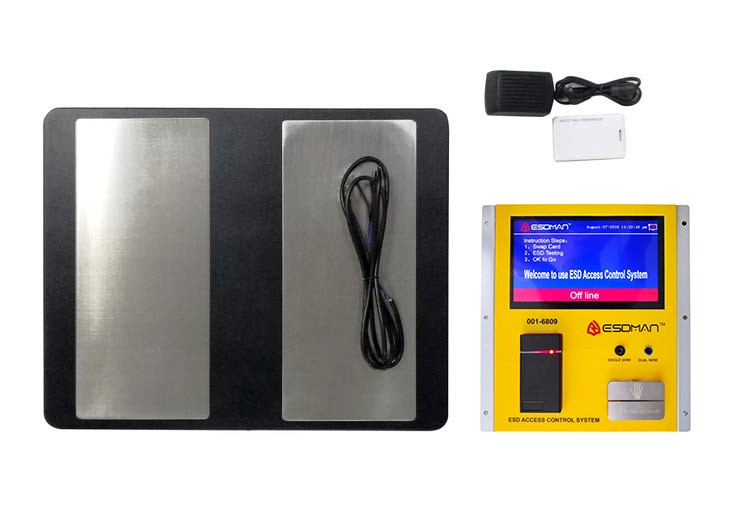
\includegraphics[width=\textwidth]{pics/SAL4_05.jpg}
                \caption{ESDMAN Access Control System \cite{ESDMAN_0016809}}
                \label{fig:fig1}
            \end{subfigure}
            \hfill
            \begin{subfigure}[t]{0.45\textwidth}
                \centering
                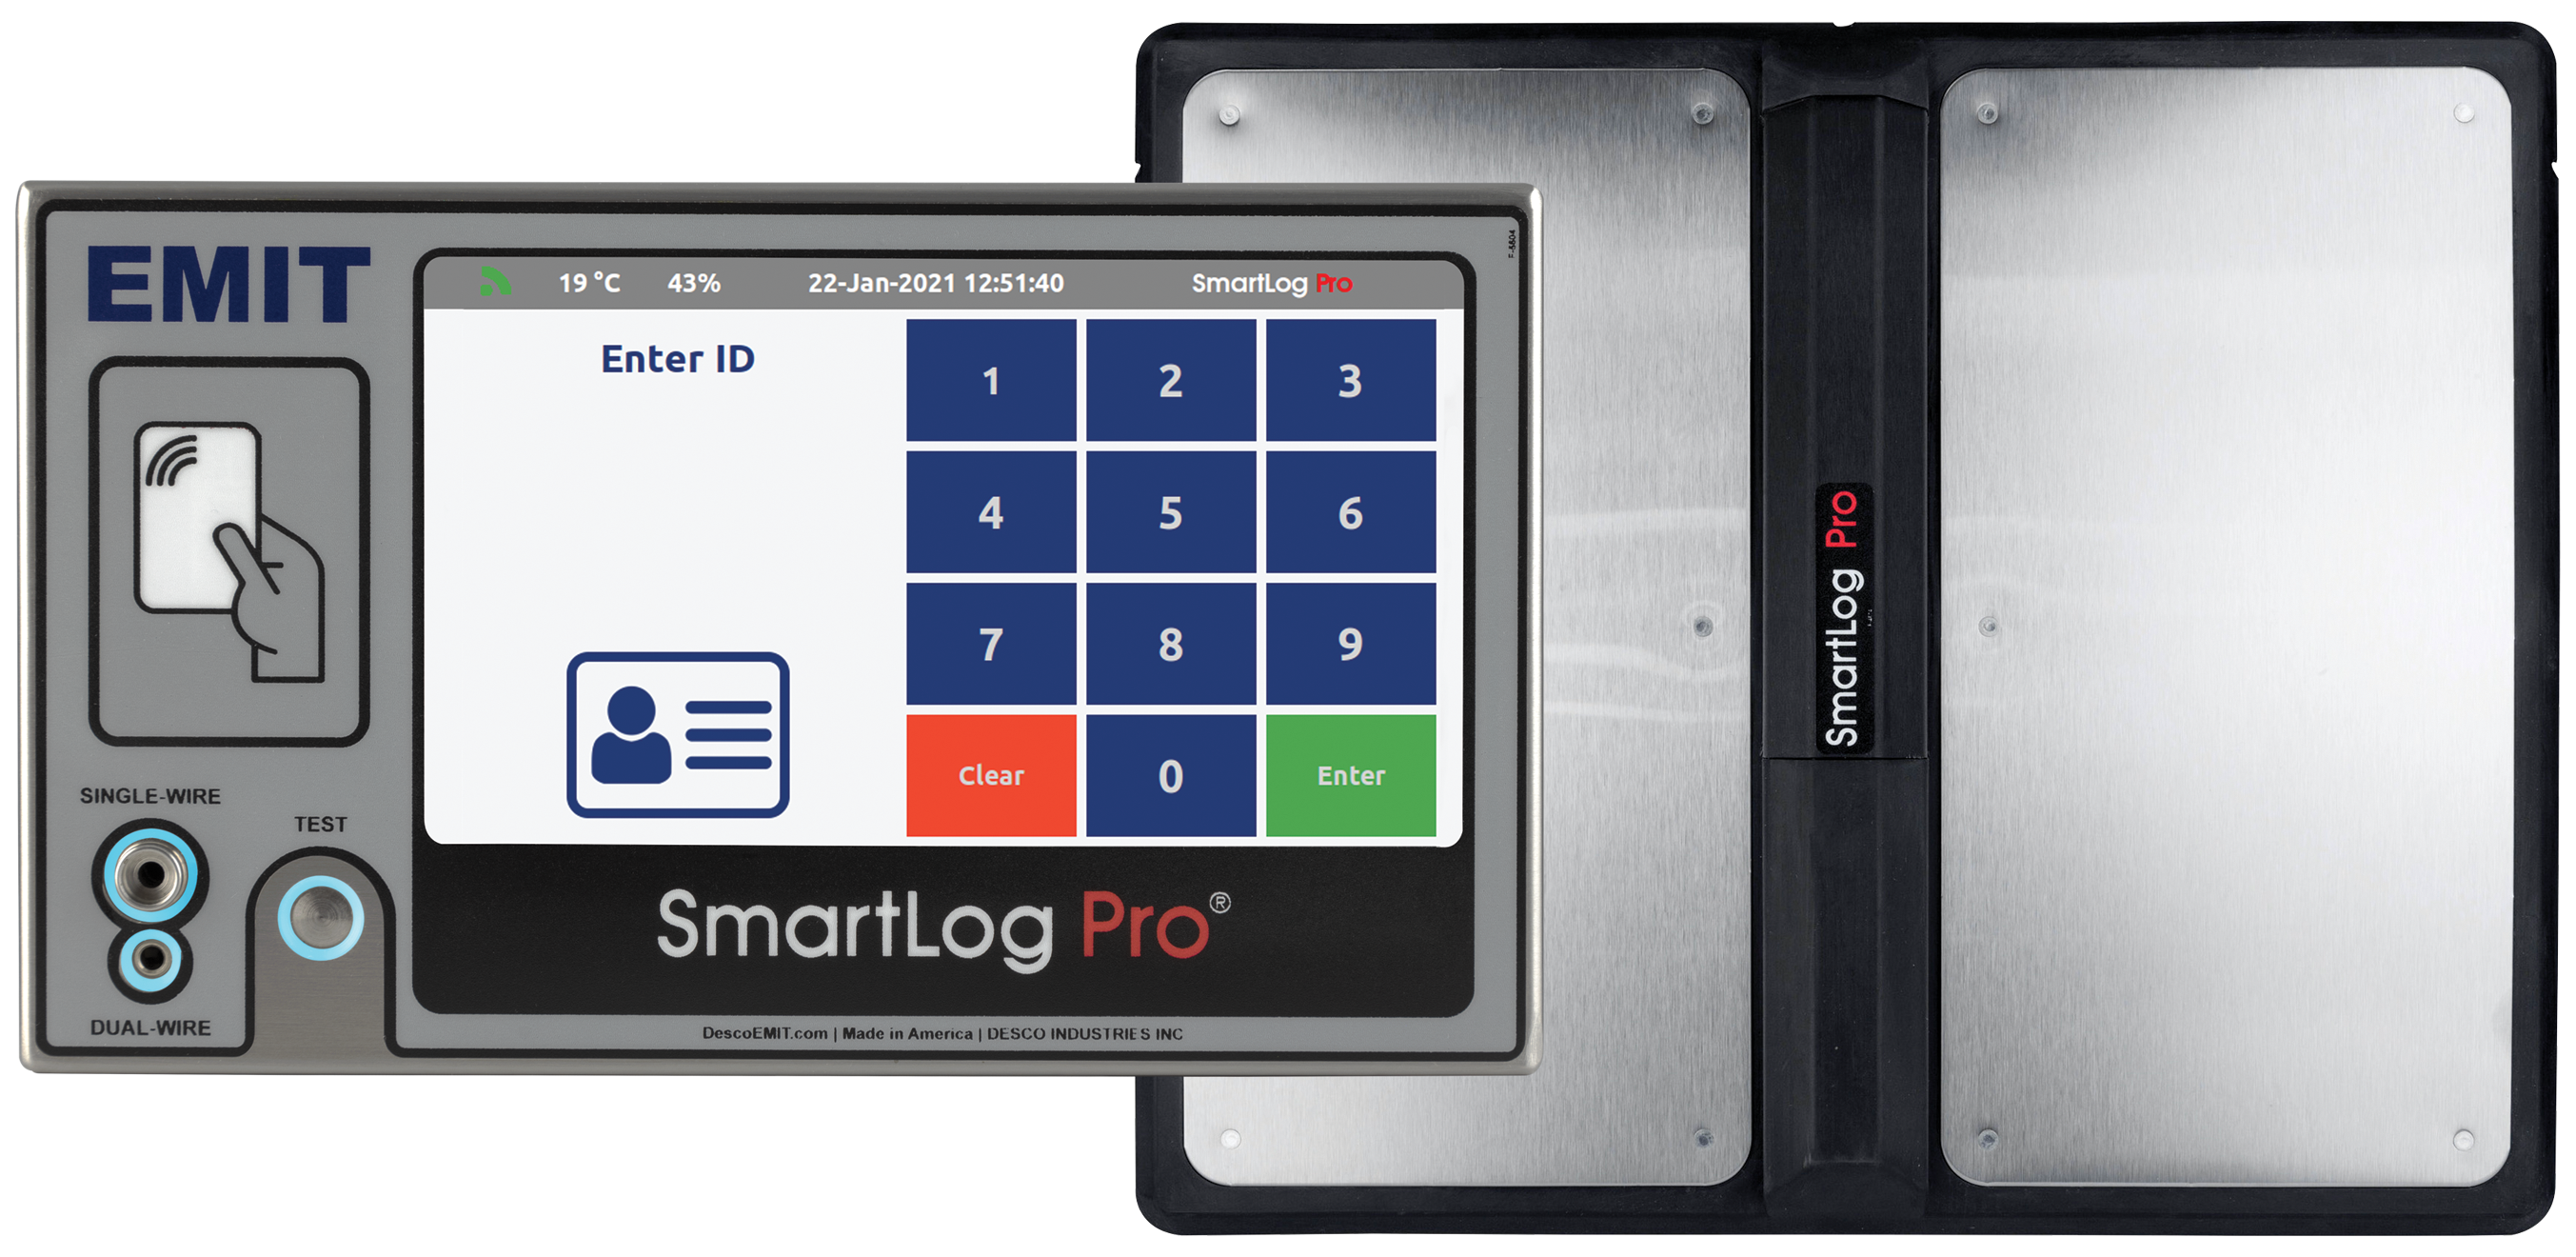
\includegraphics[width=\textwidth]{pics/SAL4_06.png}
                \caption{SmartLog Pro 2 \cite{SmartLogPro2}}
                \label{fig:fig2}
            \end{subfigure}

            \caption{Sistemas de control ESD avanzados}
            \label{fig:comparacion}
        \end{figure}


    \section{Limitaciones de las soluciones existentes}
        A partir del análisis del estado del arte de se observa que no existen 
        investigaciones o articulos relevantes en el tema, a su vez no hay disponible ningún circuito front-end
        para este tipo de mediciones. Las soluciones industriales que se asemejan a el proyecto propuesto tienen
        la peculiaridad de ser costosas, no existe un producto tipo estación de control ESD que no supere los miles de 
        dolares, a su vez las soluciones en el mercado no son open source, por lo que si algun usuario desea personalizar
        el producto para sus necesidades se ve limitado a lo que ofrece el fabricante.
